\chapter{Geometry and Shrinkage}
\label{app:shrinkage}

Sometimes, it may be advantageous to incorporate ``indirect evidence'', that is, data that does not seem to be directly related to the question at hand, in order to achieve a better estimate. As a classic unintuitive example, let us briefly discuss James-Stein estimation. Suppose that over the course of the part of a season, we have gathered data on the batting averages of baseball players, and would like to predict their performance in the rest of the season. At first glance, it would seem that from the data alone, our best shot is to estimate each player's average independently, since the players themselves should perform independently of each other. However, the statistical world in 1955 received a shocking result from Charles Stein: he proved that by ``shrinking'' each individual average toward the grand mean, it is possible to obtain a lower total squared error in higher dimensional scenarios \cite{Stein_1956}. Although our focus is not quite the same thing as this particular estimation problem, we will see that the idea of shrinkage is a rather natural way to view what we were trying to do in \cref{ch:atrds}, especially once we consider a more geometric interpretation of points along a statistical manifold.

\section{Geometric Interpretation}

Back in \cref{ch:atrds}, at one step, we separately learned many different posterior distributions for each day in our dataset, and essentially combined all of this information together by learning a mapping from a label generated from contextual information and observed outcome, to a common representative posterior for a particular group of labels. This can naturally be broken up into two steps: first, clustering our many candidate distributions into meaningful groups, and second, using these groupings in combination to learn something useful together. We will call these the clustering step and combination step in the rest of this chapter, though we note that they do not necessarily have to be done separately, as we did them together earlier. However, the process that we derived was rather complicated and involved. Fortunately, in this section, and the rest of the chapter, we will introduce a more interpretable formulation. We will use it as a canvas for further directions of study, although we will not be going into as much technical detail, and will instead focus on discussing ideas.

\subsection{Natural Statistical Manifold}

To simplify the problem a bit for now, we will treat all of our contextual information, including weather, under a single $y$ variable, and include all of our observation information under a single $x$ variable. Then, we can associate each point $c=(x,y)$ in our dataset, each corresponding to a day of flights, to a learned posterior distribution for $z$, which we will call $\qvd{z;c}$. In this way, we can define a statistical manifold parameterized by $c=(x,y)$, in which each point is associated with its own probability distribution \cite{Matsuzoe_2010}, as seen in \cref{fig:example-statistical-manifold}.

\begin{figure}[htb!]
    \centering
    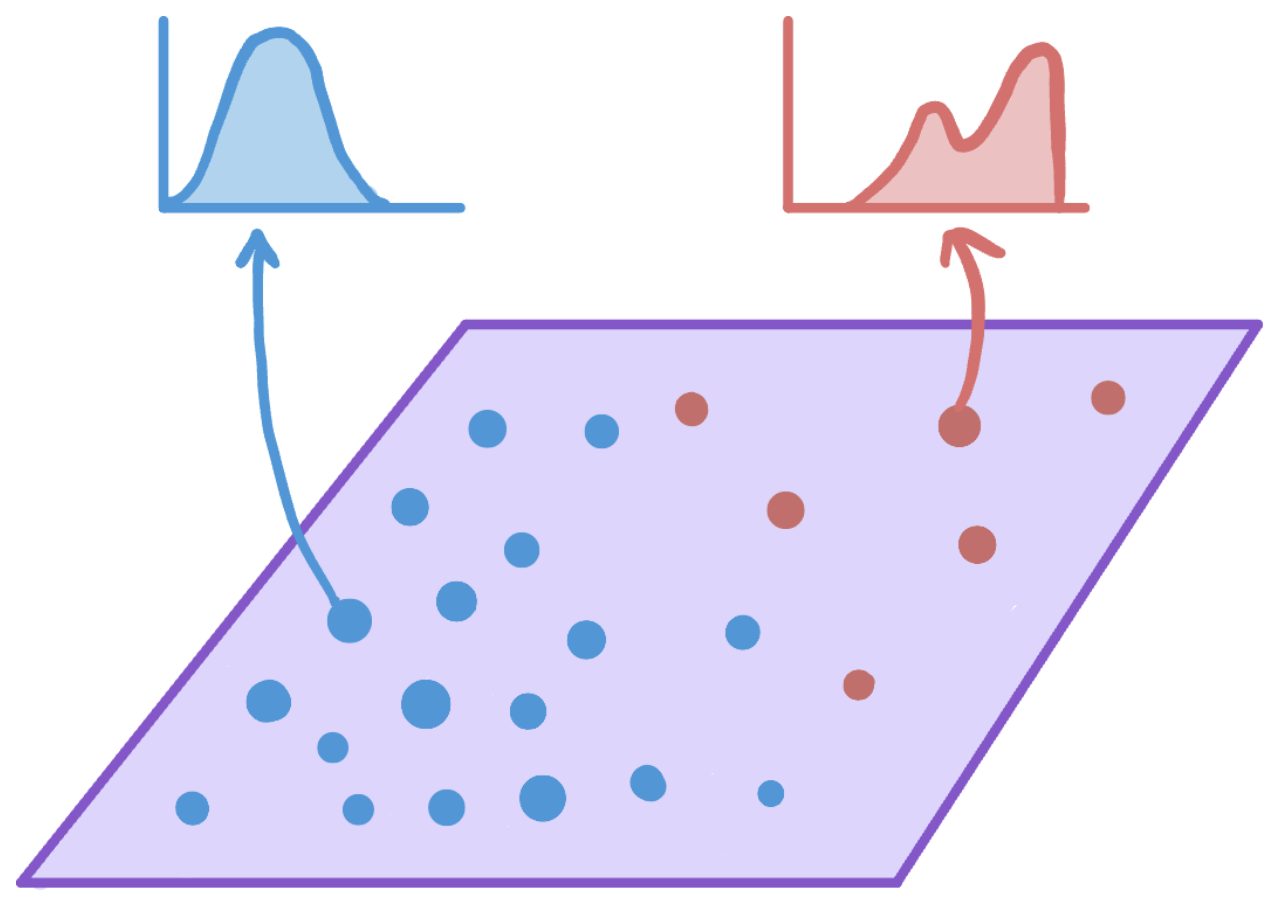
\includegraphics[width=0.5\linewidth]{media/example-statistical-manifold.png}
    \caption{An example of a statistical manifold.}
    \label{fig:example-statistical-manifold}
\end{figure}


This sort of interpretation is useful for working under an information geometric perspective. In particular, if we adopt the Fisher information metric, log-likelihood as we used earlier can be considered as a differentiable map \cite{Murray_Rice_1993}. The choice of metric is flexible, however, and depending on application, we may also want use other options such as the Wasserstein metric, which is related to optimal transport \cite{bigot2019statisticaldataanalysiswasserstein}. Note that we do not actually have access to the entire manifold. Instead, we just have observations corresponding to points on it, along with an approximated learned distribution, and we make the assumption that the latent underlying manifold is smooth. It is also useful for visualization purposes, as it can be easier to think about what we are doing with points on an object when thinking about the clustering and combination steps, than trying to directly reason with the actual mathematical objects. 

\section{Self-regularization as Shrinkage}

In this section, we will assume that we have the clustering step already taken care of, so that our data is already neatly separated into groups that we now want to work with. We have already seen a sort of self-regularization in our guiding case study in \cref{ch:atrds}, but now, we will adopt and extend an existing framework to cover our previous use case and more. In particular, we will also attempt to provide a shrinkage based reinterpretation.

\subsection{Calibrated Normalizing Flows}

First, we briefly recap the problem formulation and method as presented in the \CALNF{} work in \cite{dawson2025rare}. Rare event modeling is formulated as a data-constrained Bayesian inverse problem, where the goal is to infer the posterior distribution of latent variables $z$ from observations $\rx\sim \pld{x\given z;y}$, where $y$ are known context variables. 

\begin{example}[\CALNF{} Problem Formulation]
    We have nominal observations $\Data_0 = \{x_0^{(i)}, y_0^{(i)}\}_{i=1}^{N_0}$ and much fewer target observations $\Data_t = \{x_t^{(i)}, y_t^{(i)}\}_{i=1}^{N_t}$ available, where $N_t \ll N_0$. We wish to learn an approximation for the posterior distribution of $z$ for the target (anomaly or failure) data:
    \begin{equation}
        \qvd{z} \approx \pld{z\given \Data_t} = \pld{z\given \{x_t^{(i)}, y_t^{(i)}\}_{i=1}^{N_t}}.
    \end{equation}
\end{example}

Specifically, we use variational inference, and aim to maximize the evidence lower bound (ELBO) given by
\begin{equation}
    \elbo{}{\phi, \theta, \Data} = \EX{(x,y)\in \Data}{ \EX{z\sim \qvd{z}}{\log\pld{x,z;y}-\log\qvd{z}} }
\end{equation}
To deal with the limited target data available, \CALNF{} then adopts a bootstrapping inspired approach, where the target data $\Data_t$ is resampled into $K$ subsets $\Data_t^{(1)},\ldots,\Data_t^{(K)}$, and instead aims to learn a conditional normalizing flow $\qvd{z;c}$ where one-hot labels $c=\vone_i$ correspond to each of the target subset $\Data_t^{(i)}$, zero label $c=\vzero_K$ corresponds to the nominal data $\Data_0$, and $c^*$ is a desired optimal label representing the best mixture of the various $\qvd{z;\vone_i}$ to approximate $\qvd{z;c^*}\approx \pld{z\given \Data_t}$. 

\begin{proposition}[\CALNF{} Objective]
    The optimization problem is given by $\phi^*, c^* = \argmin_{\phi, c} L(\phi, c)$, where the loss is
    \begin{equation}
        \label{eq:calnf-loss}
        \underbrace{\beta\sum_{i\ne j} \DKL{\qvd{\cdot;\vone_i}}{\qvd{\cdot;\vone_j}}}_{\substack{\mathstrut\text{TSSO}\mathstrut\\\text{(Target Subset Similarity)}}}
        -\underbrace{\frac1K \sum_{i=1}^K \elbo{}{\phi,\theta,\Data_t^{(i)};\vone_i}}_{\substack{\mathstrut\text{TSMO}\mathstrut\\\text{(Target Subset Matching)}}}
        -\underbrace{\elbo{}{\phi,\theta,\Data_0;\vzero_K}}_{\substack{\mathstrut\text{NMO}\mathstrut\\\text{(Nominal Matching)}}}
        -\underbrace{\elbo{}{\phi,\theta,\Data_t;c}}_{\substack{\mathstrut\text{TMO}\mathstrut\\\text{(Target Matching)}}}
    \end{equation}
    where we write the mixture label $c$-specific ELBO as
    \begin{equation}
        \elbo{}{\phi, \theta, \Data; c} = \EX{(x,y)\in \Data}{ \EX{z\sim \qvd{z;c}}{\log\pld{x,z;y}-\log\qvd{z;c}} }.
    \end{equation}
\end{proposition}

\subsection{Split Likelihood Objectives}

We can see how each goal is incorporated into the overall objective $L(\phi,c)$. The last three terms in \cref{eq:calnf-loss} are the target subset matching objective (TSMO), nominal matching objective (NMO), and the target matching objective (TMO), which aim to maximize the ELBO on each target subset with labels $\vone_i$, the nominal data with label $\vzero_K$, and target data with label $c^*$, respectively. The first term is the target subset similarity objective (TSSO), which encourages similarity between the target subset posteriors, in the sense of small total pairwise KL-divergence. It is also shown that learning the mapping from labels $c$ to the candidate distributions for the posterior approximation implicitly regularizes the Wasserstein distance between the learned nominal and calibrated target posteriors.

However, although the influence of hyperparameter tuning is lessened compared to standard prior regularization methods, empirical results also showed that this learning process can be sensitive to $\beta$ in the TSSO. Specifically, empirical results showed that when the failure dataset was very small, larger values of $\beta$ which encourage similarity perform better, and when the failure dataset was larger, smaller values of $\beta$ which allow for more diversity perform better. Additionally, there are also essentially hyperparameters for the weights of the TSMO, NMO, and TMO, which are fixed at one, but this may not always be entirely appropriate.

One way we might be able to eliminate these hyperparameters entirely is by developing a principled way to specify how related the nominal data with label, target data, and target subsets, should be to each other. As we will discuss in a later section, when additional contextual information for the latent parameters is available, it can be the source of informing these similarities, though it may also be worth considering ways to do so with the current setting, such as by attempting to formalize the empirical relationship between optimal $\beta$ and relative failure and nominal dataset size.

\subsection{Generalized Calibrated Normalizing Flows}

Before we address these challenges, we will briefly consider a generalization of the \CALNF{} setup to work with multiple possibly related regimes, instead of just a simple nominal and target split. This will be relevant to our air traffic problem, as we may have many different failures modes and even different nominal modes. Therefore, consider the following generalized formulation.

\begin{example}[Generalized \CALNF{} Problem Formulation]
    We have observations $\Data_k = \{x_k^{(i)}, y_k^{(i)}\}_{i=1}^{N_k}$ for $m$ different regimes enumerated from $1$ to $k$. We wish to learn an approximation for the posterior distribution of $z$ under each regime:
    \begin{equation}
        \qvd{z} \approx \pld{z\given \Data_k} = \pld{z\given \{x_k^{(i)}, y_k^{(i)}\}_{i=1}^{N_k}}, \qquad k=1,2,\ldots,m.
    \end{equation}
\end{example}

Note that the original formulation also falls under this, as we assumed we already had sufficient data to approximate the posterior for $\Data_0$ on its own. Additionally, we could have considered each of the resampled subsets as datasets from very similar regimes, though we knew it should have been the same since they were all from the same target distribution. 

This time, we will assign labels $c_k$ to each dataset, which do not necessarily have to be the one-hot target and zero nominal encoding from before. Now, we can build the loss again, step-by-step. First, we have a direct analogue for all of the matching objectives, TSMO, NMO, and TMO, as simply the mixture label $c_k$-specific ELBO for each dataset, with an appropriate weight applied. Tackling the similarity objective, TSSO, is a bit more complicated, because may no longer be appropriate to place equal weight on the similarity for all pairs. For now, we will leave these as hyperparameters, and show how we might select them in a way that makes sense.

\begin{proposition}[Generalized \CALNF{} Objective]
    The optimization problem is given by $\phi^*, c^* = \argmin_{\phi, c} L(\phi, c)$, where the loss is
    \begin{equation}
        \label{eq:gen-calnf-loss}
        L(\phi, c) =
        \underbrace{\sum_{i\ne j} s_{i,j}\cdot \DKL{\qvd{\cdot;i}}{\qvd{\cdot;c_j}}}_{\substack{\mathstrut\text{RSO}\mathstrut\\\text{(Regime Similarity)}}}
        -\underbrace{\sum_{k=1}^m m_k\cdot \elbo{}{\phi,\theta;c_k}}_{\substack{\mathstrut\text{RMO}\mathstrut\\\text{(Regime Matching)}}}
    \end{equation}
    and we write the regime $k$-specific ELBO as
    \begin{equation}
        \elbo{}{\phi, \theta; k} = \EX{(x,y)\in \Data_k}{ \EX{z\sim \qvd{z;c_k}}{\log\pld{x,z;y}-\log\qvd{z;c_k}} }.
    \end{equation}
    Here, $s_{i,j}$ and $m_k$ are weights applied to each term in their respective objective.
\end{proposition}

Of course, one simple way to choose weights, as before, is to set all $m_k=1$ and all $s_{i,j}=\beta$. For an appropriate choice of $\beta$, or a very small value, this won't even necessarily perform abysmally, because the Regime Matching Objective (RMO) can do much of the heavy lifting if needed and if we aren't totally lacking in data for all sets. When we are lacking data, we can also still use the bootstrapping-inspired approach from the original formulation, as we can take the objectives corresponding to a target subset and split them up like before. We do have to be careful, however, about adding too many, as we may run into computational efficiency issues from having to run calculations for so many more pairings and subsets.

\begin{example}[Generalized \CALNF{} Objective with Target Subsets]
    Without loss of generality, suppose that $1,2,\ldots, l$ are target subsets that we wish to apply the resample approach to. Then, directly adding in the relevant objectives yields
    \begin{align}
        \label{eq:gen-calnf-loss-one-target}
        &\phantom{+}
        \underbrace{\sum_{i\ne j} s_{i,j}\cdot \DKL{\qvd{\cdot;c_i,\vzero_K}}{\qvd{\cdot;c_j,\vzero_K}}}_{\substack{\mathstrut\text{RSO}\mathstrut\\\text{(Regime Similarity)}}}
        -\underbrace{\sum_{k=1}^m m_k\cdot \elbo{}{\phi,\theta;k,0}}_{\substack{\mathstrut\text{RMO}\mathstrut\\\text{(Regime Matching)}}} \\
        &+ \underbrace{\sum_{k=1}^l\beta_k \spars*{
        \sum_{i\ne j} \DKL{\qvd{\cdot;c_k,\vone_i}}{\qvd{\cdot;c_k,\vone_j}}}}_{\substack{\mathstrut\text{RTSSO}\mathstrut\\\text{(Regime Target Subset Similarity)}}}
        -\underbrace{\sum_{k=1}^l \spars*{\frac{m_k}K \sum_{i=1}^K \elbo{}{\phi,\theta;k,i}} }_{\substack{\mathstrut\text{RTSMO}\mathstrut\\\text{(Regime Target Subset Matching)}}}.
    \end{align}
\end{example}

Here, we extend each label by length $K$ to augment the regime label $c_k$ with a subset label $\vone_i$ or a nominal $\vzero_K$, and adjust the granular ELBO $\elbo{}{\cdot}$ definition accordingly.

\subsection{Shrinkage Perspective}

First, going back to the original \CALNF{} formulation, the idea of prior regularization using the nominal distribution can be viewed as shrinking the learned target distribution toward the learned nominal distribution, or essentially moving to a closer point on the statistical manifold. Similarly, the resampled target subsets also experience shrinking toward each other through the similarity objective. Our generalization follows a similar idea, as we are now concerned with how much we should be shrinking each point toward each other, as controlled by the $m_k$ and $s_{i,j}$ weights.

\section{Identifying Related Failures}

In the previous section, we mainly focused on the combination step, and introduced some generalizations that required setting some hyperparameters related to similarity of different pairs of failure modes, or regimes, and of their relative influence individually. 

One case is when we already have prior distributions on the latent parameters $z$ specified. In this case, we can use the similarities of these distributions to inform what our similarity pair weights $s_{i,j}$ should be. For example, if our prior belief is that we expect regimes $i$ and $j$ to be more similar, which may be expressed by similar prior distributions for both of them, we should place a higher weight on their similarity terms. Similarly, the confidence expressed by the priors can also help inform the choice of individual influence weights $m_k$. Prior distributions that are less dispersed represent greater confidence in the belief, and so it would make sense to place a higher weight on the corresponding matching term. In our guiding case study, we had already looked into specifying prior distributions, so this was something that was sort of implicitly done during the process, albeit a bit differently.

In the remainder of this shorter section, we will also briefly discuss some ideas for when we do not immediately have this information available, and may need to work with the data only. As such, we will also focus more on the clustering step at first, since figuring out how to split our data into groups that likely come from similar distributions will help in our understanding of this problem.

\subsection{Clustering Learned Posteriors}

Let us return to our initial geometric formulation for a moment, where we have learned approximate posteriors $\qvd{z;c}$ for a collection of points $c=(x,y)$ on our statistical manifold. This is, in fact, a rather convenient representation, because as long as we have some notion of distance between two points $c_1$ and $c_2$, in a way that aligns with the similarity of their associated distributions, we can directly perform existing hierarchical clustering methods \cite{Ran_Xi_Lu_Wang_Lu_2023}. Note that our framework in \cref{ch:atrds} essentially implicitly clusters the individual per-day posteriors as part of its process, so this is something we have sort of already been doing. 

Because the structure of our data may be rather complicated, especially as we move from the single airport case to full network case, capturing the similarity between distributions may also become more difficult than before. In this case, it could also be worth applying Topological Data Analysis (TDA) methods, which attempt to extract this sort of information in a more robust manner, by studying the ``shape'' of data in a rigorous sense \cite{chazal2021introductiontopologicaldataanalysis}.

\subsection{Integrating Credibility Weighting}

One final idea we will discuss is again relevant for selecting the $m_k$ weights for our generalized \CALNF{} objective. As we mentioned earlier, the original authors found that encouraging similarity performed better for small target datasets, but for larger datasets, allowing diversity was preferable. One way we can attempt to formalize this idea and apply it to our individual influence weights is by using ideas from credibility theory. Roughly speaking, we can compare the variance of the expected values of a group, which we call the Variance of Hypothetical Mean (VHM), and the expected variance over all groups, which we call the Expected Value of the Process Variance (EVPV). Using these, we assign a credibility to the data from a group, which we can consider as analogous to our $m_k$ weights that are assigned to each dataset. Credibility decreases as EVPV increases, and increases as VHM increases. We will not go into much more detail here, as the main intent was to mention the idea of assigning importance based on the makeup of their contributions to the total variance, in terms of VHM and EVPV \cite{Buhlmann_1967}.

\section{Summary}

In this chapter, we introduced a more natural geometric interpretation of our original inference problem by viewing it as working with points on a statistical manifold. We then saw how this interpretation naturally lends itself to a shrinkage view in a generalized \CALNF{} framework for posterior approximation. Finally, we briefly discussed some clustering and credibility methods, which could be useful for setting up natural groups and weights for our generalized \CALNF{} objective.